% $Header: /cvsroot/latex-beamer/latex-beamer/examples/beamerexample5.tex,v 1.22 2004/10/08 14:02:33 tantau Exp $

\documentclass[11pt]{beamer}

\usetheme{Darmstadt}

\usepackage{times}
\usefonttheme{structurebold}

%\usepackage[english]{babel}
\usepackage[brazilian]{babel}
\usepackage{pgf,pgfarrows,pgfnodes,pgfautomata,pgfheaps}
\usepackage{amsmath,amssymb}
\usepackage[utf8]{inputenc}
%\usepackage[latin1]{inputenc}
\usepackage{graphicx}
\usepackage{tikz}
\usepackage{cancel}
\usetikzlibrary{arrows.meta, positioning, calc}
\setbeamercovered{dynamic}

\newcommand{\Lang}[1]{\operatorname{\text{\textsc{#1}}}}

\newcommand{\Class}[1]{\operatorname{\mathchoice
  {\text{\sf \small #1}}
  {\text{\sf \small #1}}
  {\text{\sf #1}}
  {\text{\sf #1}}}}

\newcommand{\NumSAT}      {\text{\small\#SAT}}
\newcommand{\NumA}        {\#_{\!A}}

\newcommand{\barA}        {\,\bar{\!A}}

\newcommand{\Nat}{\mathbb{N}}
\newcommand{\Set}[1]{\{#1\}}

\pgfdeclaremask{tu}{beamer-tu-logo-mask}
\pgfdeclaremask{computer}{beamer-computer-mask}
\pgfdeclareimage[interpolate=true,mask=computer,height=2cm]{computerimage}{beamer-computer}
\pgfdeclareimage[interpolate=true,mask=computer,height=2cm]{computerworkingimage}{beamer-computerred}
\pgfdeclareimage[mask=tu,height=.5cm]{logo}{logounesp}

\logo{\pgfuseimage{logo}}

\title{Análise Combinatória e Probabilidades}
\author{Ney Lemke}
\institute[IBB-UNESP]{%
    Departamento de Biofísica e Farmacologia}
\date{\today}

\colorlet{redshaded}{red!25!bg}
\colorlet{shaded}{black!25!bg}
\colorlet{shadedshaded}{black!10!bg}
\colorlet{blackshaded}{black!40!bg}

\colorlet{darkred}{red!80!black}
\colorlet{darkblue}{blue!80!black}
\colorlet{darkgreen}{green!80!black}

\def\radius{0.96cm}
\def\innerradius{0.85cm}

\def\softness{0.4}
\definecolor{softred}{rgb}{1,\softness,\softness}
\definecolor{softgreen}{rgb}{\softness,1,\softness}
\definecolor{softblue}{rgb}{\softness,\softness,1}

\definecolor{softrg}{rgb}{1,1,\softness}
\definecolor{softrb}{rgb}{1,\softness,1}
\definecolor{softgb}{rgb}{\softness,1,1}

\newcommand{\Bandshaded}[2]{
  \color{shadedshaded}
  \pgfmoveto{\pgfxy(-0.5,0)}
  \pgflineto{\pgfxy(-0.6,0.1)}
  \pgflineto{\pgfxy(-0.4,0.2)}
  \pgflineto{\pgfxy(-0.6,0.3)}
  \pgflineto{\pgfxy(-0.4,0.4)}
  \pgflineto{\pgfxy(-0.5,0.5)}
  \pgflineto{\pgfxy(4,0.5)}
  \pgflineto{\pgfxy(4.1,0.4)}
  \pgflineto{\pgfxy(3.9,0.3)}
  \pgflineto{\pgfxy(4.1,0.2)}
  \pgflineto{\pgfxy(3.9,0.1)}
  \pgflineto{\pgfxy(4,0)}
  \pgfclosepath
  \pgffill

  \color{black}  
  \pgfputat{\pgfxy(0,0.7)}{\pgfbox[left,base]{#1}}
  \pgfputat{\pgfxy(0,-0.1)}{\pgfbox[left,top]{#2}}
}

\newcommand{\Band}[2]{
  \color{shaded}
  \pgfmoveto{\pgfxy(-0.5,0)}
  \pgflineto{\pgfxy(-0.6,0.1)}
  \pgflineto{\pgfxy(-0.4,0.2)}
  \pgflineto{\pgfxy(-0.6,0.3)}
  \pgflineto{\pgfxy(-0.4,0.4)}
  \pgflineto{\pgfxy(-0.5,0.5)}
  \pgflineto{\pgfxy(4,0.5)}
  \pgflineto{\pgfxy(4.1,0.4)}
  \pgflineto{\pgfxy(3.9,0.3)}
  \pgflineto{\pgfxy(4.1,0.2)}
  \pgflineto{\pgfxy(3.9,0.1)}
  \pgflineto{\pgfxy(4,0)}
  \pgfclosepath
  \pgffill

  \color{black}  
  \pgfputat{\pgfxy(0,0.7)}{\pgfbox[left,base]{#1}}
  \pgfputat{\pgfxy(0,-0.1)}{\pgfbox[left,top]{#2}}
}

\newcommand{\BaenderNormal}
{%
  \pgfsetlinewidth{0.4pt}
  \color{black}
  \pgfputat{\pgfxy(0,5)}{\Band{input tapes}{}}
  \pgfputat{\pgfxy(0.35,4.6)}{\pgfbox[center,base]{$\vdots$}}
  \pgfputat{\pgfxy(0,4)}{\Band{}{}}

  \pgfxyline(0,5)(0,5.5)
  \pgfxyline(1.2,5)(1.2,5.5)
  \pgfputat{\pgfxy(0.25,5.25)}{\pgfbox[left,center]{$w_1$}}

  \pgfxyline(0,4)(0,4.5)
  \pgfxyline(1.8,4)(1.8,4.5)        
  \pgfputat{\pgfxy(0.25,4.25)}{\pgfbox[left,center]{$w_n$}}
  \ignorespaces}

\newcommand{\BaenderZweiNormal}
{%
  \pgfsetlinewidth{0.4pt}
  \color{black}
  \pgfputat{\pgfxy(0,5)}{\Band{Zwei Eingabebänder}{}}
  \pgfputat{\pgfxy(0,4.25)}{\Band{}{}}

  \pgfxyline(0,5)(0,5.5)
  \pgfxyline(1.2,5)(1.2,5.5)
  \pgfputat{\pgfxy(0.25,5.25)}{\pgfbox[left,center]{$u$}}

  \pgfxyline(0,4.25)(0,4.75)
  \pgfxyline(1.8,4.25)(1.8,4.75)        
  \pgfputat{\pgfxy(0.25,4.5)}{\pgfbox[left,center]{$v$}}
  \ignorespaces}

\newcommand{\BaenderHell}
{%
  \pgfsetlinewidth{0.4pt}
  \color{black}
  \pgfputat{\pgfxy(0,5)}{\Bandshaded{input tapes}{}}
  \color{shaded}
  \pgfputat{\pgfxy(0.35,4.6)}{\pgfbox[center,base]{$\vdots$}}
  \pgfputat{\pgfxy(0,4)}{\Bandshaded{}{}}

  \color{blackshaded}
  \pgfxyline(0,5)(0,5.5)
  \pgfxyline(1.2,5)(1.2,5.5)
  \pgfputat{\pgfxy(0.25,5.25)}{\pgfbox[left,center]{$w_1$}}

  \pgfxyline(0,4)(0,4.5)
  \pgfxyline(1.8,4)(1.8,4.5)        
  \pgfputat{\pgfxy(0.25,4.25)}{\pgfbox[left,center]{$w_n$}}
  \ignorespaces}

\newcommand{\BaenderZweiHell}
{%
  \pgfsetlinewidth{0.4pt}
  \color{black}
  \pgfputat{\pgfxy(0,5)}{\Bandshaded{Zwei Eingabebänder}{}}%
  \color{blackshaded}
  \pgfputat{\pgfxy(0,4.25)}{\Bandshaded{}{}}
  \pgfputat{\pgfxy(0.25,4.5)}{\pgfbox[left,center]{$v$}}
  \pgfputat{\pgfxy(0.25,5.25)}{\pgfbox[left,center]{$u$}}%

  \pgfxyline(0,5)(0,5.5)
  \pgfxyline(1.2,5)(1.2,5.5)

  \pgfxyline(0,4.25)(0,4.75)
  \pgfxyline(1.8,4.25)(1.8,4.75)        
  \ignorespaces}

\newcommand{\Slot}[1]{%
  \begin{pgftranslate}{\pgfpoint{#1}{0pt}}%
    \pgfsetlinewidth{0.6pt}%
    \color{structure}%
    \pgfmoveto{\pgfxy(-0.1,5.5)}%
    \pgfbezier{\pgfxy(-0.1,5.55)}{\pgfxy(-0.05,5.6)}{\pgfxy(0,5.6)}%
    \pgfbezier{\pgfxy(0.05,5.6)}{\pgfxy(0.1,5.55)}{\pgfxy(0.1,5.5)}%
    \pgflineto{\pgfxy(0.1,4.0)}%
    \pgfbezier{\pgfxy(0.1,3.95)}{\pgfxy(0.05,3.9)}{\pgfxy(0,3.9)}%
    \pgfbezier{\pgfxy(-0.05,3.9)}{\pgfxy(-0.1,3.95)}{\pgfxy(-0.1,4.0)}%
    \pgfclosepath%
    \pgfstroke%
  \end{pgftranslate}\ignorespaces}

\newcommand{\SlotZwei}[1]{%
  \begin{pgftranslate}{\pgfpoint{#1}{0pt}}%
    \pgfsetlinewidth{0.6pt}%
    \color{structure}%
    \pgfmoveto{\pgfxy(-0.1,5.5)}%
    \pgfbezier{\pgfxy(-0.1,5.55)}{\pgfxy(-0.05,5.6)}{\pgfxy(0,5.6)}%
    \pgfbezier{\pgfxy(0.05,5.6)}{\pgfxy(0.1,5.55)}{\pgfxy(0.1,5.5)}%
    \pgflineto{\pgfxy(0.1,4.25)}%
    \pgfbezier{\pgfxy(0.1,4.25)}{\pgfxy(0.05,4.15)}{\pgfxy(0,4.15)}%
    \pgfbezier{\pgfxy(-0.05,4.15)}{\pgfxy(-0.1,4.2)}{\pgfxy(-0.1,4.25)}%
    \pgfclosepath%
    \pgfstroke%
  \end{pgftranslate}\ignorespaces}

\newcommand{\ClipSlot}[1]{%
  \pgfrect[clip]{\pgfrelative{\pgfxy(-0.1,0)}{\pgfpoint{#1}{4cm}}}{\pgfxy(0.2,1.5)}\ignorespaces}

\newcommand{\ClipSlotZwei}[1]{%
  \pgfrect[clip]{\pgfrelative{\pgfxy(-0.1,0)}{\pgfpoint{#1}{4.25cm}}}{\pgfxy(0.2,1.25)}\ignorespaces}


\AtBeginSection[]{\frame{\frametitle{Outline}\tableofcontents[current]}}

\begin{document}

\frame{\titlepage}

%\section*{Outline}

\part{Parte I}
\frame{\frametitle{Outline}\tableofcontents[part=1]}
\section{Probabilidades}
\frame{\frametitle{Probabilidade}
Seja um conjunto $U$ com $N$ elementos seja um subconjunto $A$ com $n_A$ 
elementos. A probabilidade de ocorrência de $A$ é
$$
p_A=\frac{n_A}{N}
$$

Exemplos:

\begin{itemize}
\item Dados
\item Cartas
\item Moedas
\end{itemize}

}

\frame{\frametitle{Eventos mutuamente Exclusivos}
Os eventos $A$ e $B$ são mutuamente exclusivos se a ocorrência de $A$ impede a ocorrência de $B$ e vice-versa. Ou seja se $A\cap B =\emptyset$.


}

\frame{\frametitle{Eventos Coletivamente Exaustivos}
Os eventos $A_1,\ldots ,A_n$ são coletivamente exaustivos se:

$$U=\cup_{i=1}^n A_i$$ 
}

\frame{\frametitle{Eventos Independentes}
Os eventos $A$ e $B$ são independentes se:

$$p_{A\cap B}=p_a p_B$$
}

\frame{\frametitle{Regra da soma}

  $$p(A \mbox { ou } B \ldots Z)=\frac{n_A+n_B+\ldots n_Z}{N}=p_A+p_B+\ldots p_Z$$
se os eventos são mutuamente exclusivos. 

}



\frame{\frametitle{Teorema}
$$p_{A\cup B}=p_A+p_B-p_{A\cap B}$$

\begin{center}
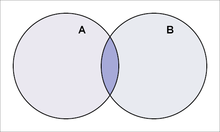
\includegraphics[scale=0.5]{intersec.png}
\end{center}
}

\frame{\frametitle{Exemplo}
Qual é a probabilidade de se obter um dado 1 no primeiro lançamento ou um dado 4 no segundo?
}
\begin{frame}
\frametitle{Problema}
\large
Qual é a probabilidade de se obter um 1 no primeiro lançamento de dado \textbf{OU} um 4 no segundo lançamento?

\begin{itemize}
\item Evento A: Obter um 1 no primeiro lançamento de dado
\item Evento B: Obter um 4 no segundo lançamento de dado
\end{itemize}

Precisamos calcular $P(A \cup B)$ - a probabilidade da união.
\end{frame}

\begin{frame}
\frametitle{Passo 1: Calcular as probabilidades individuais}
\large
\begin{itemize}
\item $P(A) = \frac{1}{6}$ 
\begin{itemize}
\item Há 1 face com o número 1 em um dado de 6 faces
\end{itemize}
\vspace{0.5cm}
\item $P(B) = \frac{1}{6}$ 
\begin{itemize}
\item Há 1 face com o número 4 em um dado de 6 faces
\end{itemize}
\end{itemize}
\end{frame}

\begin{frame}
\frametitle{Passo 2: Verificar a independência dos eventos}
\large
\begin{center}
Estes eventos ocorrem em lançamentos diferentes!
\end{center}

\vspace{0.5cm}
$\Rightarrow$ Os eventos são \textbf{independentes}

\vspace{0.5cm}
\begin{center}
Definição: Dois eventos A e B são independentes quando a ocorrência de um não influencia a probabilidade de ocorrência do outro.
\end{center}
\end{frame}

\begin{frame}
\frametitle{Passo 3: Calcular a probabilidade da interseção}
\large
Para eventos independentes:

\vspace{0.5cm}
$P(A \cap B) = P(A) \times P(B)$

\vspace{0.5cm}
$P(A \cap B) = \frac{1}{6} \times \frac{1}{6} = \frac{1}{36}$

\vspace{0.5cm}
\begin{center}
A probabilidade de obter ambos os resultados é $\frac{1}{36}$
\end{center}
\end{frame}

\begin{frame}
\frametitle{Passo 4: Aplicar a fórmula da união}
\large
Para quaisquer eventos A e B:

\vspace{0.3cm}
$P(A \cup B) = P(A) + P(B) - P(A \cap B)$

\vspace{0.5cm}
$P(A \cup B) = \frac{1}{6} + \frac{1}{6} - \frac{1}{36}$

\vspace{0.3cm}
$P(A \cup B) = \frac{6}{36} + \frac{6}{36} - \frac{1}{36}$

\vspace{0.3cm}
$P(A \cup B) = \frac{11}{36} \approx 0,306 \approx 30,6\%$
\end{frame}

\begin{frame}
\frametitle{Conclusão}
\large
\begin{center}
\textbf{A probabilidade de obter um 1 no primeiro lançamento OU um 4 no segundo lançamento é de:}

\vspace{0.5cm}
$\frac{11}{36} \approx 30,6\%$
\end{center}

\vspace{0.5cm}
\begin{itemize}
\item Esta é a aplicação direta da fórmula da união de eventos
\item Para eventos independentes, sempre calculamos $P(A \cap B) = P(A) \times P(B)$
\item Observe que $P(A \cup B) < P(A) + P(B)$ quando os eventos não são mutuamente exclusivos
\end{itemize}
\end{frame}

\begin{frame}
\frametitle{Visualização}
\large
\begin{center}
\begin{tabular}{|c|c|c|c|c|c|c|}
\hline
\multicolumn{7}{|c|}{Espaço amostral: 36 possibilidades} \\
\hline
 & \textbf{Dado 2: 1} & \textbf{Dado 2: 2} & \textbf{Dado 2: 3} & \textbf{Dado 2: 4} & \textbf{Dado 2: 5} & \textbf{Dado 2: 6} \\
\hline
\textbf{Dado 1: 1} & (1,1) & (1,2) & (1,3) & \textcolor{red}{(1,4)} & (1,5) & (1,6) \\
\hline
\textbf{Dado 1: 2} & (2,1) & (2,2) & (2,3) & \textcolor{blue}{(2,4)} & (2,5) & (2,6) \\
\hline
\textbf{Dado 1: 3} & (3,1) & (3,2) & (3,3) & \textcolor{blue}{(3,4)} & (3,5) & (3,6) \\
\hline
\textbf{Dado 1: 4} & (4,1) & (4,2) & (4,3) & \textcolor{blue}{(4,4)} & (4,5) & (4,6) \\
\hline
\textbf{Dado 1: 5} & (5,1) & (5,2) & (5,3) & \textcolor{blue}{(5,4)} & (5,5) & (5,6) \\
\hline
\textbf{Dado 1: 6} & (6,1) & (6,2) & (6,3) & \textcolor{blue}{(6,4)} & (6,5) & (6,6) \\
\hline
\end{tabular}
\end{center}

\begin{itemize}
\item \textcolor{red}{Vermelho}: $A \cap B$ (1 caso)
\item \textcolor{blue}{Azul}: Evento B sem A (5 casos)
\item Restantes em primeira linha: Evento A sem B (5 casos)
\item Total: 11 casos de 36 $\Rightarrow \frac{11}{36}$
\end{itemize}
\end{frame}

\frame{\frametitle{Probabilidade Condicional}

$p(B|A)$ denotada a probabilidade de ocorrência de $B$ dado que $A$ ocorreu.

Esta probabilidade pode ser calculada usando o teorema de Bayes:

$$p(A\cap B)=p(B|A)p(A)=p(A|B)p(B)$$

\begin{center}
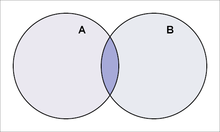
\includegraphics[scale=0.5]{intersec.png}
\end{center}

}
\section{Análise Combinatória}

\frame{\frametitle{Análise Combinatória}
  \begin{itemize}
  \item Permutações
  \item Arranjos
  \item Arranjos com Repetição
  \item Combinações
  \end{itemize}
}


\frame{\frametitle{Permutações}

  Quantas listas ordenadas contendo $n$ elementos podemos formar a
  partir de uma lista com $n$ elementos diferentes.

$$n!$$
}

\frame{\frametitle{Arranjos}

  Quantas listas ordenadas contendo $p$ elementos podemos formar a
  partir de uma lista com $n$ elementos diferentes.

$$\frac{n!}{(n-p)!}$$
}


\frame{\frametitle{Arranjos com repetição}

  Quantas listas ordenadas contendo $n$ elementos podemos formar a
  partir de uma lista com $n$ elementos, onde o elemento $e_i$ aparece repetido
$r_i$ vezes.

$$\frac{n!}{r_1!\ldots r_n!}$$
}


\frame{\frametitle{Combinações}

Quantos subconjuntos contendo $p$ elementos podemos construir com os elementos de um conjunto com $n$ elementos?

$$C_{n,p}=\frac{n!}{p!(n-p)!}$$
}

\section{Caminhante Aleatório}


\frame{\frametitle{Caminhante Aleatório}

%\begin{center}\includegraphics[scale=0.15]{rw}\end{center}
\begin{tikzpicture}[
    state/.style={circle, draw, minimum size=1cm},
    transition/.style={->, >=Stealth, bend angle=45}
]

% Estados
\node[state] (s0) at (0,0) {0};
\node[state] (s1) at (2,0) {1};
\node[state] (s2) at (4,0) {2};
\node[state] (s3) at (6,0) {3};
\node[state] (sm1) at (-2,0) {-1};
\node[state] (sm2) at (-4,0) {-2};

% Transições para a direita (probabilidade p)
\draw[transition, bend left] (sm2) to node[above] {p} (sm1);
\draw[transition, bend left] (sm1) to node[above] {p} (s0);
\draw[transition, bend left] (s0) to node[above] {p} (s1);
\draw[transition, bend left] (s1) to node[above] {p} (s2);
\draw[transition, bend left] (s2) to node[above] {p} (s3);

% Transições para a esquerda (probabilidade q)
\draw[transition, bend left] (s3) to node[below] {q} (s2);
\draw[transition, bend left] (s2) to node[below] {q} (s1);
\draw[transition, bend left] (s1) to node[below] {q} (s0);
\draw[transition, bend left] (s0) to node[below] {q} (sm1);
\draw[transition, bend left] (sm1) to node[below] {q} (sm2);

% Título e legenda
\node[above=1cm of s0] {Random Walk Unidimensional};
\node[below=1.5cm of s0] {
    \begin{tabular}{l}
        p: probabilidade de avançar \\
        q: probabilidade de retroceder \\
        p + q = 1
    \end{tabular}
};

\end{tikzpicture}
}

\frame{\frametitle{Caminhante Aleatório}
$N$ Passos

$N_1$ Passos para a frente

$N_2$ Passos para trás

Probabilidade de dar $N_1$ passos para a frente.
$$W_N(N_1)=\frac{N!}{N_1! (N-N_1)!} p^{N_1} q^{N-N_1}$$
}

%\frame{\frametitle{Caminhante Aleatório}
%Temos que:
%
%$$\sum_{N_1=0}^N W_N(N_1)=\sum_{N_1=0}^N \frac{N!}{N_1! (N-N_1)!} p^{N_1} q^{N-N_1}=(p+q)^N=1$$
%
%É conveniente investigar a posição do caminhante $m=N_1-N_2$. Neste caso
%
%$$W_N(m)=\frac{N!}{\left( \frac{N+m}{2}\right)!\left( \frac{N-m}{2}\right)!} p^{N_1} q^{N-N_1}$$
%}
%
%\frame{\frametitle{Equação Estocástica}
%
%$$P_N(m)=pP_{N-1}(m-1)+q P_{N-1}(m+1)$$
%
%Considere o caso $p=q=1/2$
%
%$$\frac{P_{N+\tau}-P_N}{\tau}\sim \frac{\partial P}{\partial t}$$
%
%$$\frac{P_N(ml-l)+P_N(ml+l)-2 P_N(ml)}{l^2}\sim \frac{\partial^2 P}{\partial x^2}$$
%
%Equação da Difusão:
%
%$$\frac{\partial P}{\partial t}=D\frac{\partial^2 P}{\partial x^2}$$
%}
\frame{\frametitle{Equação da Difusão}
A equação da difusão descreve o espalhamento de partículas em um meio devido ao movimento aleatório.
Pode ser derivada a partir de um modelo estocástico simples.
}

\frame{\frametitle{Modelo Estocástico}
Considere um sistema unidimensional onde a partícula se move para a direita ou para a esquerda com probabilidades iguais:
\begin{equation}
P_N(m) = \frac{1}{2} P_{N-1}(m-1) + \frac{1}{2} P_{N-1}(m+1)
\end{equation}
}

\frame{\frametitle{Equação da Difusão}


\begin{center}
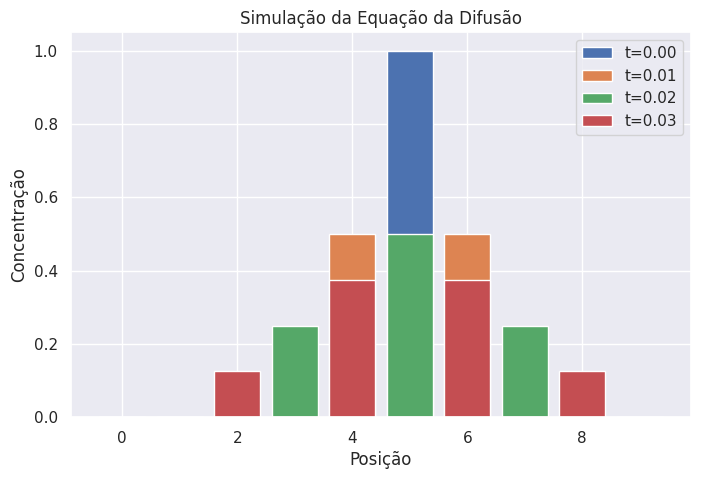
\includegraphics[scale=0.5]{eqdifusao.png}
\end{center}

}

\frame{\frametitle{Aproximação Contínua no Tempo}


\begin{equation}
P_N(m) - P_{N-1}(m)= \frac{1}{2} P_{N-1}(m-1) + \frac{1}{2} P_{N-1}(m+1)-P_{N-1}(m)
\end{equation}

\begin{equation}
  x=m\times l \quad t=N\times \tau 
\end{equation}
\begin{equation}
\frac{P_{N} - P_{N-1}}{\tau} \approx \frac{\partial P}{\partial t}
\end{equation}
}

\frame{\frametitle{Aproximação Contínua no Espaço}
\begin{equation}
\frac{P_N(m-1) + P_N(m+1) - 2P_N(m)}{l^2} \approx \frac{\partial^2 P}{\partial x^2}
\end{equation}
}

\frame{\frametitle{Equação da Difusão}
Combinando as aproximações temporais e espaciais:
\begin{equation}
\frac{\partial P}{\partial t} = D \frac{\partial^2 P}{\partial x^2}
\end{equation}
Onde o coeficiente de difusão é dado por:
\begin{equation}
D = \frac{l^2}{2\tau}
\end{equation}
}


\frame{\frametitle{Valores Médios}
Seja $u_j$ uma variável estocástica que pode assumir $N$ valores.

$$\sum^N P(u_j)=1$$

$$\langle u \rangle =\sum^Nu_jP(u_j)$$

$$(\Delta u)^2=(u-\langle u \rangle)^2=\langle u^2\rangle-\langle u\rangle^2 $$

}


\frame{\frametitle{Caminhante Aleatório}


$$\langle N_1 \rangle = \sum_{N_1} N_1 W_N(N_1)=\sum_{N_1} N_1 \frac{N!}{N_1! (N-N_1)!} p^{N_1} q^{N-N_1}$$

$$\langle N_1 \rangle = p\frac{\partial}{\partial p} \sum_{N_1} W_N(N_1)=\sum_{N_1} N_1 \frac{N!}{N_1! (N-N_1)!} p^{N_1} q^{N-N_1}$$

$$\langle N_1 \rangle=p\frac{\partial}{\partial p}(p+q)^N$$

$$\langle N_1 \rangle =pN(p+q)^{N-1}=pN$$

$$\langle N_2 \rangle=\langle N-N_1 \rangle=N(1-p)=Nq$$
}

\frame{\frametitle{Caminhante Aleatório}
$$\langle N_1^2 \rangle=p\frac{\partial}{\partial p}p\frac{\partial}{\partial p} \sum_{N_1}  W_N(N_1)=\sum_{N_1} N_1^2 \frac{N!}{N_1! (N-N_1)!} p^{N_1} q^{N-N_1}$$

$$\langle N_1^2 \rangle= p\frac{\partial}{\partial p}p\frac{\partial}{\partial p}(p+q)^N=pN+p^2N(N-1)$$

$$(\Delta N_1)^2=\langle N_1^2\rangle-\langle N_1\rangle^2 $$

$$(\Delta N_1)^2=pN+p^2N(N-1)-p^2N^2=Np(1-p)=Npq$$

$$\Delta N_1=\sqrt{Npq}$$
}

\frame{\frametitle{Lei dos Grandes Números}
$$\frac{\Delta N_1}{\langle N_1\rangle }=\sqrt{\frac{q}{pN}}$$
\begin{center}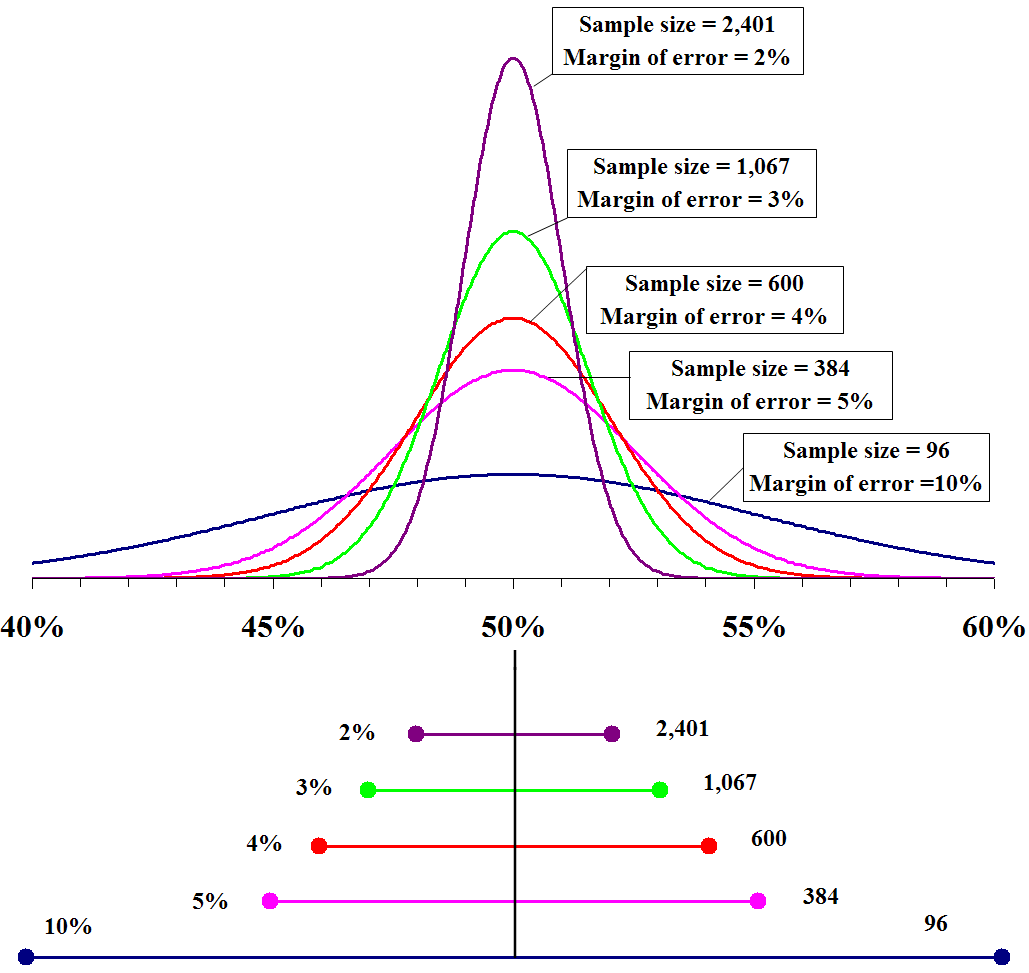
\includegraphics[scale=0.1]{lln.png}\end{center}

}
\begin{frame}
\frametitle{Introdução à Fórmula de Stirling}
\begin{itemize}
\item Aproximação assintótica para fatoriais:
\[ N! \approx \sqrt{2\pi N} \left( \frac{N}{e} \right)^N \]
\item Forma logarítmica:
\[ \ln N! \approx N \ln N - N + \frac{1}{2} \ln N + \ln \sqrt{2\pi} \]
\item Aplicações: termodinâmica, mecânica estatística, teoria das probabilidades.
\end{itemize}
\end{frame}


\begin{frame}{Introdução}
  \begin{itemize}
    \item Começamos com a definição:
      \[
      \ln N! = \sum_{k=1}^{N} \ln k.
      \]
    \item Nosso objetivo é obter uma aproximação assintótica para $\ln N!$, que, ao ser exponenciada, fornecerá a famosa fórmula:
      \[
      N! \sim \sqrt{2\pi N}\, N^N e^{-N}.
      \]
  \end{itemize}
\end{frame}

\begin{frame}{Aproximação pela Integral}
  \begin{itemize}
    \item Uma aproximação inicial é substituir a soma por uma integral:
      \[
      \sum_{k=1}^{N} \ln k \approx \int_{1}^{N} \ln x\,dx.
      \]
    \item Calculando a integral:
      \[
      \int_{1}^{N} \ln x\,dx = \left[ x\ln x - x \right]_1^N = N\ln N - N + 1.
      \]
    \item Assim, temos:
      \[
      \ln N! \sim N\ln N - N.
      \]
  \end{itemize}
\end{frame}

\begin{frame}{Aprimoramento via Euler-Maclaurin}
  \begin{itemize}
    \item Para refinar a aproximação, utilizamos a fórmula de Euler-Maclaurin:
      \[
      \sum_{k=a}^{b} f(k) \approx \int_{a}^{b} f(x)\,dx + \frac{f(a)+f(b)}{2} + \cdots.
      \]
    \item Para $f(x)=\ln x$, obtemos:
      \[
      \ln N! \approx \int_{1}^{N} \ln x\,dx + \frac{\ln 1 + \ln N}{2} + \cdots.
      \]
    \item Como $\ln 1=0$, isso se simplifica para:
      \[
      \ln N! \approx N\ln N - N + 1 + \frac{1}{2}\ln N + \cdots.
      \]

  \end{itemize}
\end{frame}
      
\begin{frame}{Aprimoramento via Euler-Maclaurin}
  \begin{itemize}
    \item Ajustando a constante (e considerando termos de ordem superior), chega-se à forma:
      \[
      \ln N! \sim N\ln N - N + \frac{1}{2}\ln(2\pi N).
      \]
  \end{itemize}
\end{frame}

\begin{frame}{Fórmula de Stirling}
  \begin{itemize}
    \item Exponenciando ambos os lados, obtemos:
      \[
      N! \sim \sqrt{2\pi N}\, N^N e^{-N}.
      \]
    \item Esta é a famosa Fórmula de Stirling, amplamente utilizada em estatística, física e teoria dos números.
  \end{itemize}
\end{frame}



\begin{frame}
\frametitle{Método de Laplace: Intuição Geométrica}
\begin{itemize}
\item Propósito: Avaliar integrais do tipo
\[ \int_a^b e^{M f(x)} dx \quad (M \gg 1) \]
\item Ideia-chave: O integrando é dominado por uma região estreita em torno do máximo de \( f(x) \).

\item Passos principais:
\begin{enumerate}
\item Localizar o ponto de máximo \( x = c \).
\item Expandir \( f(x) \) em série de Taylor até segunda ordem.
\item Reduzir o integral a um gaussiano.
\end{enumerate}
\end{itemize}
\end{frame}

\begin{frame}
\frametitle{Aplicação à Função Gama}
\begin{itemize}
\item Representação integral do fatorial:
\[ N! = \int_0^\infty x^N e^{-x} dx \]
\item Reescrevendo o integrando:
\[
N! = \int_0^\infty e^{N \ln x - x} dx = \int_0^\infty e^{M f(x)} dx
\]
onde \( M = N \), \( f(x) = \ln x - \frac{x}{N} \).
\end{itemize}
\end{frame}

\begin{frame}
  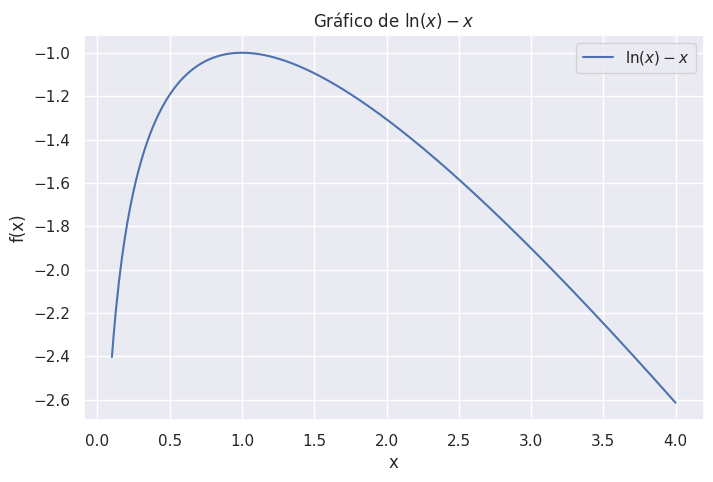
\includegraphics[scale=0.5]{laplace.png}
\end{frame}

\begin{frame}
\frametitle{Passo 1: Encontrar o Máximo}
\begin{itemize}
\item Derivada primeira:
\[ f'(x) = \frac{1}{x} - \frac{1}{N} \]
\item Ponto crítico: \( x_c = N \)
\item Derivada segunda no máximo:
\[ f''(N) = -\frac{1}{N^2} \quad (< 0 \Rightarrow \text{máximo}) \]
\end{itemize}
\begin{center}
    \textit{A função tem um pico estreito em \( x = N \).}
\end{center}
\end{frame}

\begin{frame}
\frametitle{Passo 2: Expansão de Taylor}
\begin{itemize}
\item Expandir \( f(x) \) em torno de \( x = N \):
\[
f(x) \approx f(N) + \cancelto{0}{f'(N)(x-N)} + \frac{f''(N)}{2}(x-N)^2
\]
\[
f(x) \approx \ln N - 1 - \frac{(x-N)^2}{2N^2}
\]
\item Fator exponencial dominante:
\[
e^{N f(x)} \approx e^{N (\ln N - 1)} e^{-\frac{(x-N)^2}{2N}}
\]
\end{itemize}
\end{frame}

\begin{frame}
\frametitle{Passo 3: Substituição de Variáveis}
\begin{itemize}
\item Nova variável adimensional:
\[ t = \frac{x - N}{\sqrt{N}} \quad \Rightarrow \quad dx = \sqrt{N} dt \]
\item Limites de integração:
\[ x = 0 \Rightarrow t = -\sqrt{N} \quad (\text{desprezível para } N \gg 1) \]
\[ \int_0^\infty \to \int_{-\infty}^\infty \text{ para aproximação} \]
\item Integral transformada:
\[
N! \approx e^{N \ln N - N} \sqrt{N} \int_{-\infty}^\infty e^{-t^2/2} dt
\]
\end{itemize}
\end{frame}

\begin{frame}
\frametitle{Passo 4: Integral Gaussiana}
\begin{itemize}
\item Identidade fundamental:
\[ \int_{-\infty}^\infty e^{-t^2/2} dt = \sqrt{2\pi} \]
\item Resultado final:
\[
N! \approx e^{N \ln N - N} \sqrt{N} \cdot \sqrt{2\pi}
\]
\[
N! \approx \sqrt{2\pi N} \left( \frac{N}{e} \right)^N
\]
\end{itemize}
\end{frame}

\begin{frame}
  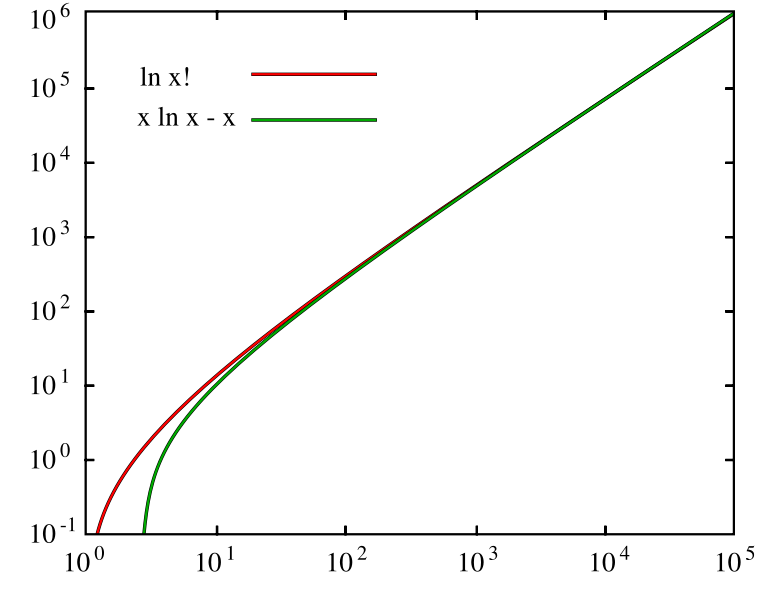
\includegraphics[scale=0.5]{stirling.png}
\end{frame}
\begin{frame}
\frametitle{Conclusão e Observações}
\begin{itemize}
\item Método de Laplace captura: 
\begin{itemize}
\item Termo dominante \( \left( \frac{N}{e} \right)^N \)
\item Correção subdominante \( \sqrt{2\pi N} \)
\end{itemize}

\item Erro relativo decai como \( \mathcal{O}(1/N) \)
\item Generalizações:
\begin{itemize}
\item Expansões de ordem superior (Wallis, Euler-Maclaurin)
\item Aplicações em sistemas com muitos graus de liberdade
\end{itemize}
\end{itemize}
\end{frame}



%\frame{\frametitle{Aproximação de Stirling}
%
%$$\ln N!=\ln 1+\ldots \ln N\sim \int_1^N \ln x\, d x=N \ln N -N +1\sim N\ln N -N $$
%
%
%ou ainda 
%
%$$N!\sim \sqrt{2\pi N}\left( \frac{N}{e} \right)^N$$
%
%\begin{center}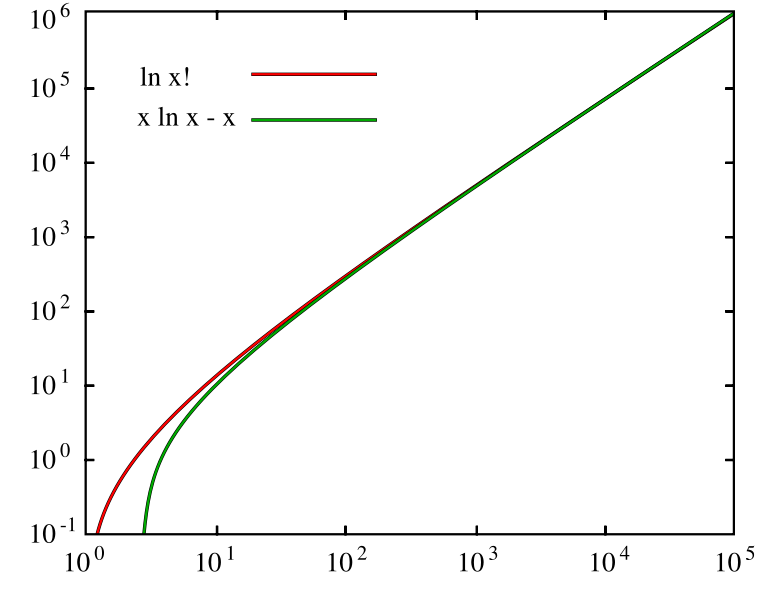
\includegraphics[scale=0.1]{stirling.png}\end{center}
%}

\frame{\frametitle{Limite Gaussiano}

$$f(N_1)=\ln W_N(N_1) =ln N!-\ln N_1 - \ln N_2!+N_1\ln p+N_2 \ln q$$

Usando a aproximação de Stirling:

$$f(N_1)=N\ln N-N_1\ln N_1-(N-N_1)\ln (N-N_1)+N_1\ln p +(N-N_1)\ln q$$

Expansão em torno do máximo $N_1^*$:

$$f(N_1)\sim f(N_1^*)+(N_1-N_1^*)^2\left. \frac{1}{2}\frac{\partial^2 f}{\partial N_1^2}\right|_{N_1=N_1^*}+\ldots$$
}

\frame{\frametitle{Limite Gaussiano}
Equação para o máximo:

$$\frac{\partial f}{\partial N_1}=0$$

$$-\ln N_1^*+\ln (N_1-N_1^*)+\ln p-\ln q=0$$

$$N_1^*=N p$$
}
\frame{\frametitle{Limite Gaussiano}

Também precisamos calcular:

$$\frac{\partial^2 f}{\partial N_1^2}=\frac{1}{N-N_1}-\frac{1}{N_1}$$

$$\left. \frac{\partial^2 f}{\partial N_1^2}\right|_{N_1=N_1^*}=\frac{-1}{Npq}$$

$$f(N_1)\sim\ln W_N(N_1^*)-\frac{-(N_1-Np)^2}{2 Npq}$$

Normalizando temos que:

$$p(N_1)=\frac{1}{\sqrt{2 \pi N p q}}
\exp\left( \frac{-(N_1-Np)^2}{2 Npq}\right)$$
}

\end{document}
